\chapter{Fundamentação Teórica}
\label{chap:fundteor}

% \begin{flushright}

%    \begin{list}{}{
%       \setlength{\leftmargin}{4.5cm}
%       \setlength{\rightmargin}{0cm}
%       \setlength{\labelwidth}{0pt}
%       \setlength{\labelsep}{\leftmargin}}
%       \item Quanto maior for a rapidez de transformação de uma
%       sociedade, mais temporárias são as necessidades
%       individuais. Essas flutuaçõess tornam ainda mais acelerado
%       o senso de turbilh da sociedade.

%       \begin{list}{}{
%       \setlength{\leftmargin}{0cm}
%       \setlength{\rightmargin}{0cm}
%       \setlength{\labelwidth}{0pt}
%       \setlength{\labelsep}{\leftmargin}}
%       \item (Alvin Toffler)
%       \end{list}
%    \end{list}
% \end{flushright}

% \begin{flushright}
%   Quanto maior for a rapidez de transformação de uma \\
%   sociedade, mais temporárias são as necessidades \\
%   individuais. Essas flutuações tornam ainda mais \\
%   acelerado o senso de turbilhão da sociedade. \\
%   \ \\
%   (Alvin Toffler)
% \end{flushright}

%--------- NEW SECTION ----------------------
\section{Estudo da Odometria}
Informações relacionadas a localização são essenciais em diversas aplicações relacionadas à robótica móvel nos dias atuais. Determinar a posição em um ambiente, dado um mapa daquele ambiente e dados sensoriais locais, pode ser a definição de localização para um robô móvel. Isto foi um dos grandes problemas passados na área de robótica e ainda nos tempos atuais é um campo de bastante estudo.
Como uma das possíveis soluções para este problema, foi apresentado o cálculo baseado em medidas odométricas. Odometria nada mais é que o uso de dados capturados por sensores de movimento e assim então estimar mudança de posição com o tempo. É altamente usada na robótica por alguns robôs com rodas ou legados para estimar sua posição relativa de um ponto de partida. Entretanto, para um uso efetivo desta tecnologia é necessário uma captura rápida e precisa de dados, calibração de instrumentos e processamento.

Um sensor interessante para captura de dados como velocidade e posição é o sensor de WiFi. Um exemplo prático foram pesquisadores da Universidade da Carolina do Norte desenvolveram um meio para capturar a velocidade e distância em ambientes indoor através de um sensor WiFi. Este sensor funciona como um sensor de velocidade para assim rastrear com precisão o quão longe algo se moveu; exatamente como um sonar mas usando ondas de rádio ao invés de ondas de som.
\cite{Diego2016}

\begin{itemize}

    \item \textbf{Trilateração}: métodos que utilizam as propriedades geométricas do triângulo para encontrar a posição do alvo. Diferente da triangulação, este processo determina o posicionamento a partir de 3 pontos de referência diferentes, assim como acontece em sistemas de GPS(Global Positioning System). Podem ser divididos em métodos por lateração e angulação.;
    
    \begin{itemize}
        \item \textbf{Lateração} estima a posição do objeto através da leitura de distâncias a partir de múltiplos pontos de referência.
        
        \begin{itemize}
            \item \textbf{TOA (Time Of Arrival)}: a distância do alvo móvel até a unidade medidora
            é diretamente proporcional ao tempo de propagação; 
            \item \textbf{TDOA (Time Difference Of Arrival)}: este método busca determinar a posição relativa do transmissor através da diferença de tempo entre o envio até as unidades recptoras.
            \item \textbf{Baseadas em RSS (Received Signal Strength)}: método que calcula a distância baseada na atenuação da força do sinal entre o emissor e o receptor. Os métodos baseados em RSS, assim como os dois anteriores necessitam da inexistência de obstáculos físicos entre os participantes da conversa.
            \item \textbf{RTOF (Reflection Time Of Flight)}: este método utiliza do valor de Time of Flight, ou tempo de voo do sinal, para estimar a posição. O tempo de voo do sinal 
            \item \textbf{RSP (Received Signal Phase)}: utiliza a diferença de fase no sinal das portadoras (de telefonia, por exemplo) para estimar a posição.
        \end{itemize}

        \item \textbf{Angulação}: estima a posição do alvo através da interseção de vários pares de
        ângulos das linhas de direção. Cada linha é formada pelo raio do círculo de alcance
        do sinal partindo da estação base ao receptor móvel.

    \end{itemize}

    \item \textbf{Análise de Cenário}: refere-se aos métodos que primeiro recuperam características do sinal de Wi-Fi no ambiente e depois estimam a localização de um objeto através da relação da informação do sinal atual junto ao sinal adquirido anteriormente. 

\end{itemize}

A complexidade das iterações do sinal de Wi-Fi em ambientes fechados favorece a utilização dos métodos baseados em mapas, orientados por dados de intensidade do sinal.
Deixando a utilização da odometria por Wi-Fi menos optável. Biswas e Veloso propôem um método onde a posição é estimada em um processo de duas etapas. Chamados de fase de aprendizado e fase de localização.
A primeira define-se como a construção de um mapa na forma de um grafo, onde cada vértice armazena um conjunto de médias e desvios padão das forças do sinal de cada ponto de acesso Wi-Fi mensurada naquela posição e cada aresta do mapa representa um caminho possível para movimentação do robô.
E a segunda, utiliza um algoritmo que se baseia em filtro de partículas para a obtenção da posição do robô, relacionando as medições do sinal Wi-Fi recebido durante a movimentação com os valores previamente populados no mapa.\cite{Biswas2010}

%--------- NEW SECTION ----------------------
\section{Aplicação na Robótica}
\label{sec:ass1} 
As aplicações de sensores Wi-Fi encontradas na pesquisa feita para esse artigo utilizam o sensor como complemento na localização \textit{indoor} de robôs móveis. 
\textit{Micro Aerial Vehicles} (MAVs) podem usar \textit{access points} (APs) de conexão para auxiliar na localização e navegação autônoma \cite{Zhang2020}.
\cite{Ito2014} usa mapas de itensidade de sinal Wi-Fi em conjunto com uma camera RGB-D para \textit{global indoor localization} e \cite{Kudo2017}
utiliza o sinal Wi-Fi para melhorar o \textit{simultaneous localization and mapping} (SLAM).
%---------------picture---------------
% \begin{figure}
%     \centering
%     \subfigure[Figure A]{\label{fig:a}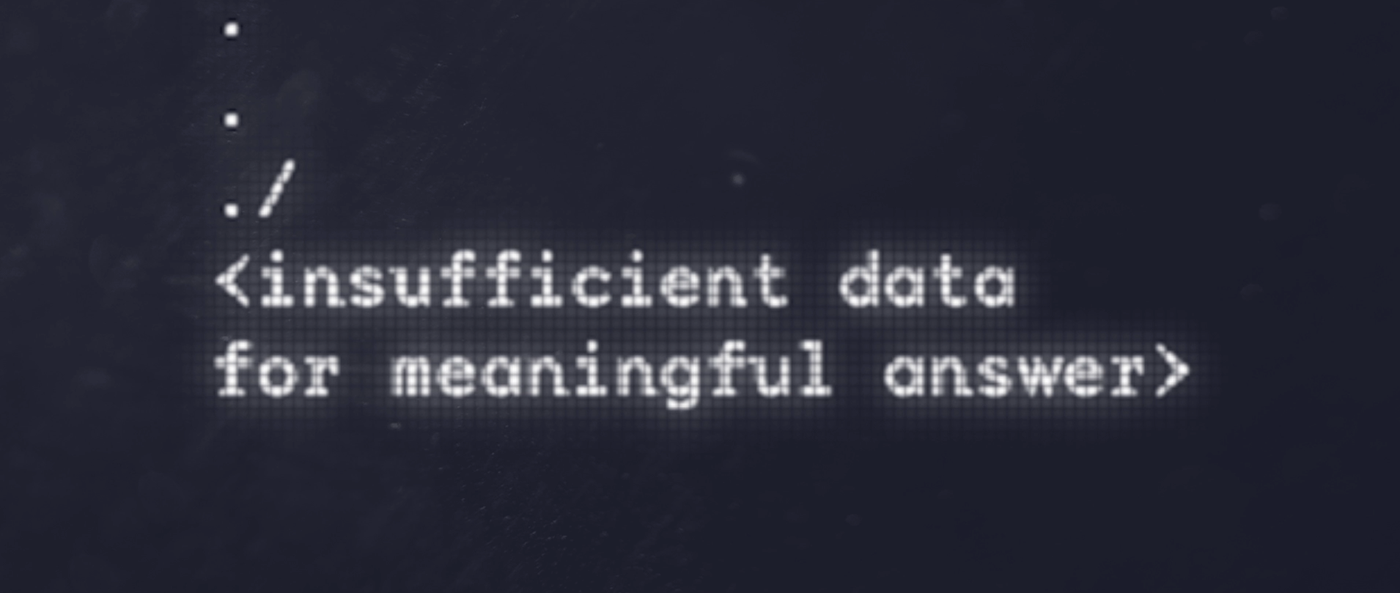
\includegraphics[width=60mm]{./lq}}
%     \subfigure[Figure B]{\label{fig:b}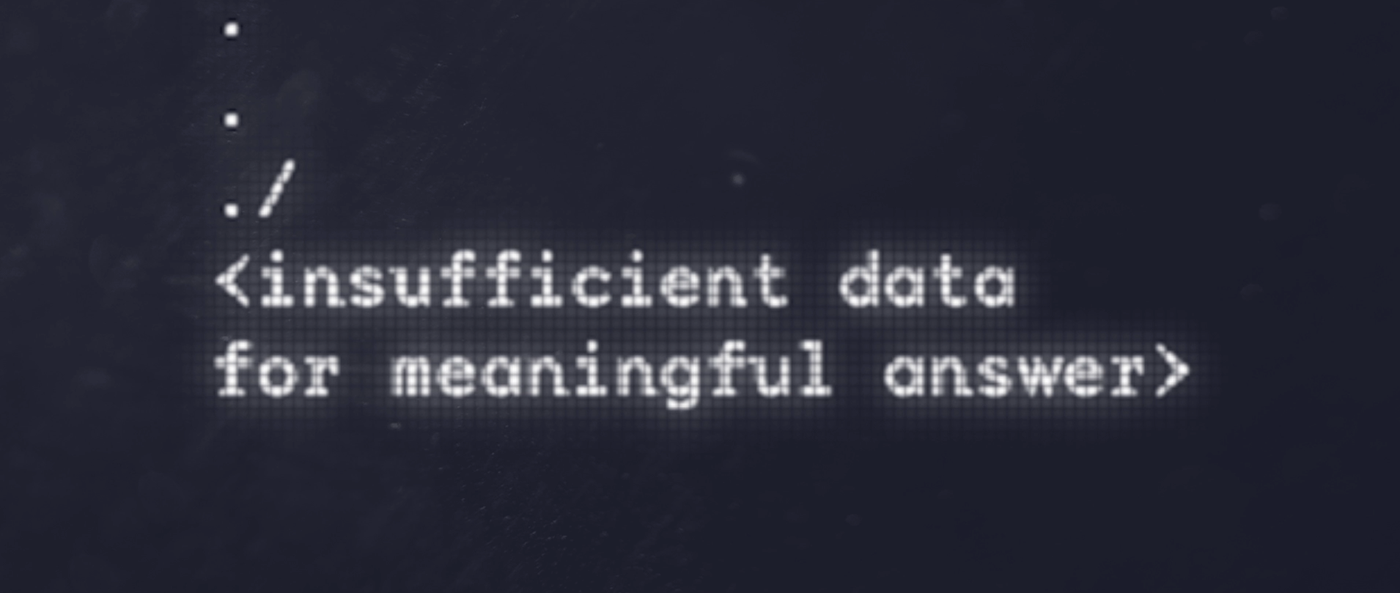
\includegraphics[width=60mm]{./lq}}
%     \subfigure[Figure C]{\label{fig:c}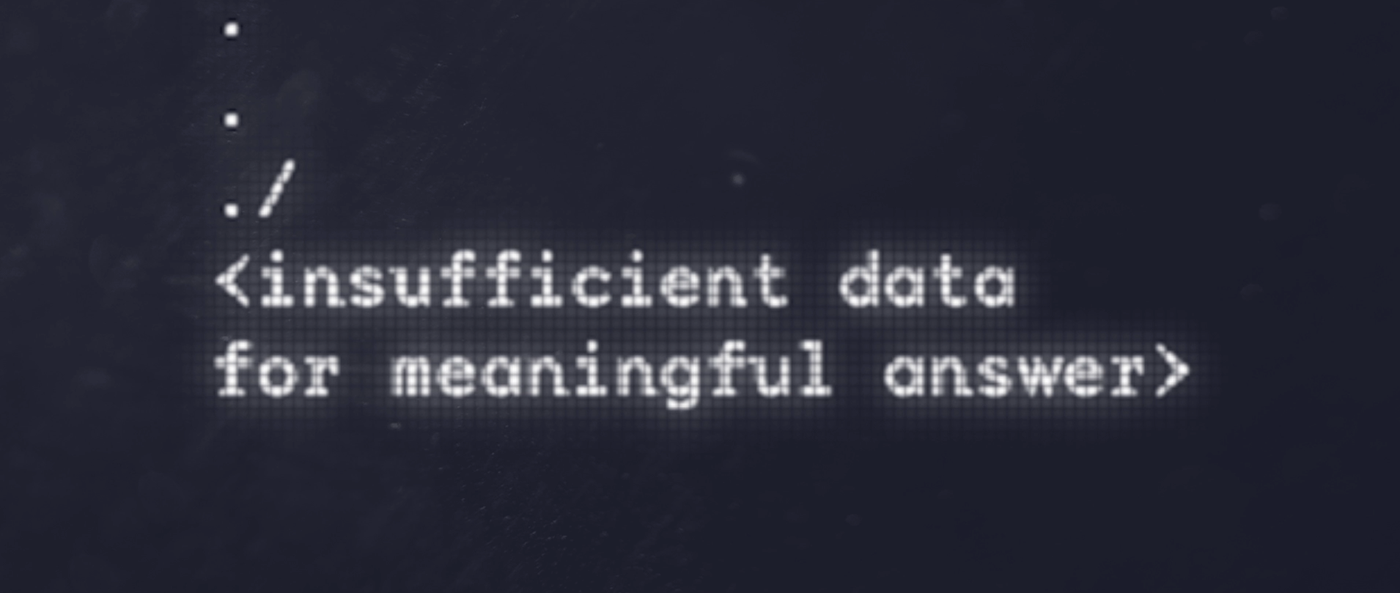
\includegraphics[width=\textwidth]{./lq}}
%     \caption{Three simple graphs}
%     \label{fig:three graphs}
% \end{figure}
%----------------------------------------------------------

